\subsubsection{Phonetic Posteriorgrams}
A phonetic posteriorgram represents predicted framewise phoneme probabilities from a speech sample.
In this work, a pretrained acoustic model from [XX] was used, due to the high quality of the model, which had 
been trained on the extremely large and varied LibriSpeech corpus.

The acoustic model predicts 5816 senones; the dimensionality is greatly reduced by a linear discriminant 
analysis matrix, yielding the posterior probability for the 40 phonemes in the TIMIT reduced phoneme set, 
which include a silence phoneme (not a true phoneme, but essentially treated as one). Refer to the Data section for samples.


\subsubsection{Speech Synthesis from PPGs [1]}
%Text here.
To generate a mel spectrogram representation from a PPG, a modified version of Tacotron2 
was used. This worked followed NVIDIA's open-source implementation with a few modifications.
As in [XX], and as shown below, the key differences were the addition of a localized attention constraint,
which decreases the computational complexity. This is especially attractive in this case because 
the expected alignment between PPG and mel spectogram is tighter than the alignment between 
text and mel spectrogram (e.g. in the standard Tacotron2 model). Because of this, it is 
superfluous to query all encoder states.

The other important difference is that instead of an embedding layer for the input, a 
linear projection is used, since the input is not sparse, i.e. not one-hot encoded. Thus, 
each input dimension must be taken into account by the model.
The following image summarizes the architecture [XX]:

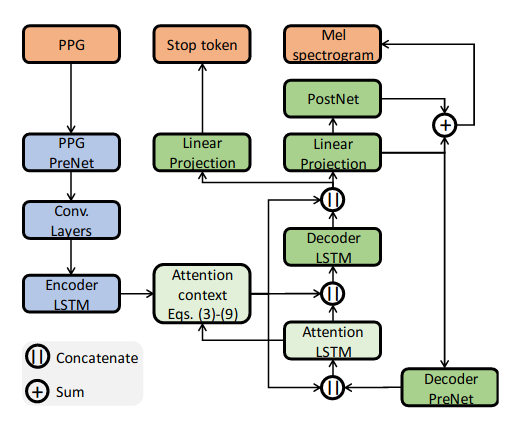
\includegraphics[width=15cm]{img/img_ppg2mel.png}


\subsubsection{Accent Transfer in PPG Space [2]}
%Text here.
Inspired by the basic architecture of MelGAN-VC, the PPG accent transfer model uses a 
generative adversarial network with a cyclical consistency constraint. 
There are two different variants.

The first architecture is convolutional, using one-dimensional convolutions across time. 
Two-dimensional convolutions were not used because there are no local spatial relationships 
across phonemes in a PPG; phoneme oder is not meaningful. The spatial relationships of interest are 
exclusively temporal. 

The second architecture is sequential, a bidirectional LSTM. Each of these 
architectures, when used, is used in both the discriminator and the generator.

*** ILLUSTRATION TO COME ***